\documentclass[a4paper, 10pt, conference]{ieeeconf}      % Use this line for a4 paper
\IEEEoverridecommandlockouts                              % This command is only needed if you want to use the \thanks command
\overrideIEEEmargins

% See the \addtolength command later in the file to balance the column lengths
% on the last page of the document

%\usepackage{fontspec}
%\setmainfont{MinionPro-Regular.otf}

% Support for changing between draft-style and published version.
\newif\ifdraft
%\drafttrue
\draftfalse

% Enable Æ
\usepackage[utf8]{inputenc}

% Enable strikethrough
\usepackage[normalem]{ulem}
% enable images
\usepackage{graphicx}


% Enable links
\usepackage{hyperref}

% Enable To-do notes
\ifdraft
	\usepackage[textsize=small]{todonotes}
	\setlength{\marginparwidth}{1.4cm} 		
\else
	\usepackage[disable]{todonotes}
\fi

% Support for drafting and sketching
\usepackage{xcolor}
\definecolor{dark-cornflower-blue-2}{RGB}{17,85,204}
\definecolor{dark-green-2}{RGB}{56,118,29}

\ifdraft
	\newcommand{\sk}[1]{{\color{dark-green-2}  #1}}
	\newcommand{\dr}[1]{{\color{dark-cornflower-blue-2} #1}}
	\newenvironment{sketch}{\color{dark-green-2}}{\ignorespacesafterend}
	\newenvironment{draft}{\color{dark-cornflower-blue-2}}{\ignorespacesafterend}
\else
	\newcommand{\sk}[1]{#1}
	\newcommand{\dr}[1]{#1}
	\newenvironment{sketch}{}{}
	\newenvironment{draft}{}{}
\fi

% Support for marking missing citations
\newcommand{\source}[0]{{\color{blue}\textsuperscript{[\textsf{\textit{need cit.}}]}}}


% Enable \cref
\usepackage{cleveref}

\usepackage[style=ieee]{biblatex}
            
% Settings for source code listings
\usepackage{listings}
\lstset{ %
  aboveskip=10pt,
  belowskip=4pt,
%  abovecaptionskip=0pt,
%  backgroundcolor=\color{white},   % choose the background color; you must add \usepackage{color} or \usepackage{xcolor}
  basicstyle=\fontsize{9pt}{10pt}\ttfamily,        % the size of the fonts that are used for the code
%  belowcaptionskip=0pt,
%  breakatwhitespace=true,         % sets if automatic breaks should only happen at whitespace
%  breakindent=17pt,
%  postbreak=\space\space,
  breaklines=true,                 % sets automatic line breaking
  captionpos=b,                    % sets the caption-position to bottom
%  commentstyle=\color{commentgray},    % comment style
%  deletekeywords={...},            % if you want to delete keywords from the given language
%  escapeinside={\%*}{*)},          % if you want to add LaTeX within your code
%  escapeinside={@}{@},
  frame=single,	                   % adds a frame around the code
%  framesep=3pt,
%  keepspaces=true,                 % keeps spaces in text, useful for keeping indentation of code (possibly needs columns=flexible)
%  keywordstyle=\color{black}\bfseries,       % keyword style
%  language=Haskell,                 % the language of the code
%  otherkeywords={Type,Vect,Nat,pure,pureM,Eff,Effect,MkEff,sig,Address,EFFECT,!,<$>,<*>,:,::},           % if you want to add more keywords to the set
  numbers=left,                    % where to put the line-numbers; possible values are (none, left, right)
  numbersep=7pt,                   % how far the line-numbers are from the code
  numberstyle=\tiny\ttfamily, % the style that is used for the line-numbers
%  rulecolor=\color{black},         % if not set, the frame-color may be changed on line-breaks within not-black text (e.g. comments (green here))
  showspaces=false,                % show spaces everywhere adding particular underscores; it overrides 'showstringspaces'
%  showstringspaces=false,          % underline spaces within strings only
%  showtabs=false,                  % show tabs within strings adding particular underscores
  stepnumber=1,                    % the step between two line-numbers. If it's 1, each line will be numbered
%  stringstyle=\color{stringmauve},     % string literal style
%  tabsize=2,	                   % sets default tabsize to 2 spaces
%  title=\lstname,                   % show the filename of files included with \lstinputlisting; also try caption instead of title
  xleftmargin=9pt,
%  xrightmargin=10pt
}


\bibliography{references}

\title{\huge Æternity blockchain\\[0.5em] \large The trustless, decentralized and purely functional oracle machine \\[1em]\today \\[1em] v0.1 }

\author{Zackary Hess \\ \href{mailto:zack@aeternity.com}{zack@aeternity.com}  
\and Yanislav Malahov \\ \href{mailto:yani@aeternity.com}{yani@aeternity.com}
\and Jack Pettersson \\ \href{mailto:jack@aeternity.com}{jack@aeternity.com} 
}

 
\begin{document}
\maketitle

\begin{abstract}

Since the introduction of Ethereum in 2014 there has been great interest in decentralized trustless applications (smart contracts). Consequently, many have tried to implement applications with real world data on top of a blockchain. We believe that storing the application's state and code on-chain is wrong for several reasons.

%blockchain architecture that is scalable, governable and scriptable. \emph{State channels} enable highly scalable, trustless transactions of value and purely functional, easily verifiable Turing-complete smart contracts. The resource-efficient consensus mechanism is aligned with the interests of the value-holders and the built-in oracle allows access to real-world data on the blockchain, which is useful for smart contracts. Applications like prediction markets and markets for synthetic assets can be efficiently implemented at global scale. Innovation is fostered via a \emph{governance} system based on \emph{futarchy}.

We present a highly scalable blockchain architecture with a consensus mechanism which is also used to check the oracle. This makes the oracle very efficient, because it avoids layering one consensus mechanism on top of another. State channels are integrated to increase privacy and scalability. Tokens in channels can be transferred using purely functional smart contracts that can access oracle answers. %, but these are only submitted to the chain in the case of dispute. 
By not storing contract code or state on-chain, we are able to make smart contracts easier to analyze and faster to process, with no substantial loss in \emph{de facto} functionality.

Applications like markets for synthetic assets and prediction markets can be efficiently implemented at global scale. Several parts have proof-of-concept implementations in Erlang. Development tools and application essentials such as a wallet, naming and identity system will also be provided.
\end{abstract}

%\pagebreak


\tableofcontents
\thispagestyle{plain} % adds numbering to pages
\pagestyle{plain} % adds with ^ numbering to pages

\section{Introduction}
\begin{draft}
The intention of this paper is to give a overview of the Æternity blockchain architecture and possible applications. More detailed papers will be released in the future, specifically for the consensus and governance mechanisms. However, it should be noted that our architecture is holistic; all components tie together and synergize, in a modular way.

The rest of this paper is broken into four parts. First, we will introduce and discuss the fundamental theoretical ideas that inform our architecture. Second, we will discuss the included essential applications, other possible use cases and give intuitions for how to use the platform as a developer. Third, we will present the current proof-of-concept implementation, written in Erlang. We conclude with a discussion, including possible future directions and comparisons to other technologies.

\subsection{Previous Work}
Blockchains, first of all Bitcoin, have shown a new way to architect value exchange on the Internet \cite{bitcoin}. This has been followed by a number of promising advances: Ethereum demonstrated a way to write Turing-complete smart contracts secured by a blockchain architecture \cite{ethereum}; Truthcoin created tools for making oracles on blockchains \cite{hivemind}, while GroupGnosis and Augur showed how to make them more efficient \cite{groupgnosis}; Casey Detrio showed how to make markets on blockchains \cite{smart-markets}; Namecoin showed how to make the distributed equivalent of a domain name server \cite{namecoin}; Factom showed how a blockchain that stores hashes can be used as a proof of existence for any digital data \cite{factom}.

These technologies show great promise when it comes to providing first-class financial and legal services to anyone. So far however, they have failed to come together to a unified whole that actually fulfills the promise. Specifically, all solutions so far have been lacking in at least one of the following respects: governance, scalability, scripting safety and cheap access to real-world data \source. Æternity aims to improve the state of the art in all of these respects.

\section{Æternity blockchain}
We believe that the lack of scalability, scripting safety and cheap access to real-world data of current ``smart contract platforms'' come down to three core issues. \emph{First}, the currently prevailing stateful design makes smart contracts written for the platform hard to analyze\footnote{The difficulty of analyzing stateful contracts was very clearly demonstrated by the re-entrance bug that brought down ``The DAO''. This happened despite the code having been audited by several of Ethereum's creators as well as the general community \source.}, and statefulness combined with sequential transaction ordering complicates scalability \source. \emph{Second}, the high cost of bringing real-world data into the system in a decentralized, trustless and reliable way complicates or outright prevents the realization of many promising applications \source. \emph{Third}, the platforms are limited in their abilities to update themselves, in order to adapt to new technological or economical knowledge. We believe that each of these three problems have clear solution paths that should be explored.

First, recent research into state channel technology suggests that for many use cases, keeping state on-chain is not necessary \source. It is very often entirely possible to store all information in state channels, and only use the blockchain to settle any economic results of the information exchange, and as a fallback in the case of dispute. This suggests an alternative approach to blockchain architecture in which Turing-complete smart contracts exist in state channels but not on-chain. This increases scalability since all transactions become independent and can thus be processed in parallel. Additionally, this means that contracts never write to shared state, greatly simplifying their testing and verification. We believe that this design emphasizes that blockchains are about financial logic rather than data storage; there exist decentralized storage solutions that complement blockchains perfectly.

Second, applications such as Augur have attempted to bring real-world data onto the blockchain in a decentralized way---in the process essentially building a consensus mechanism inside smart contracts \cite{augur}, instead of utilizing the consensus mechanism of the underlying blockchain. This leads to inefficiencies but doesn't increase security. The natural conclusion from this is to generalize the blockchain's consensus mechanism so that it can provide information not only on the next internal state, but also on the state of the external world. It could thus be argued that the blockchain's consensus mechanism determines the result of running what complexity theory dubs an \emph{oracle machine}: a theoretical machine that is more powerful than a Turing machine because it has answers to some questions that can't necessarily be computed, such as ``Who won football game X?'' \source.

Third, it seems natural that the consensus mechanism could also be used to determine the parameters of the system. This allows it to adapt to changing external conditions, as well as adopting new research and recent developments in the field.

The rest of this section introduces the Æternity blockchain in greater detail, starting with a brief overview of accounts, tokens, names and the structure of blocks. This is followed by an explanation of our approach to state channels and smart contracts, and then a discussion on how the blockchain's consensus mechanism can be used both to create an efficient oracle mechanism and to govern the system. Finally, we discuss scalability from several different angles.


\subsection{Tokens, accounts and blocks}
Despite being ``stateless'' from the contract developer's point of view, the Æternity blockchain keeps track of several predefined state components. We will now explain these, as well as the content of each block. For simplicity, this section assumes that every node keeps track of the whole blockchain. Possible optimizations are described in \cref{sec:scalability}.

\subsubsection{Access token, Aeon}
To use the blockchain is not free, but requires that the user spends a token called \emph{aeon}. Aeon are used as payment for any resources one consumes on the platform, as well as the basis for financial applications implemented on the platform. 

The distribution of aeon in the genesis block will be determined by a smart contract hosted on Ethereum. Further aeon will be created via mining.

All system fees get paid with aeon, all smart contracts settle in aeon.%Further issuance is built into the consensus, value-holders can vote to enable an issuance-transaction that requires a certain amount of proof-of-work to be valid. The cost can be updated by the consensus. % discuss if not simply the burned aeon can't be used to pay off miners (in order to keep the aeon supply constant)

\subsubsection{Accounts}
Each account has an address and a balance of aeon and also a nonce which increases with every transaction and the height of its last update. Each account also has to pay a small fee for the amount of time it is open. The costs of creating and keeping accounts prevents spam and disincentivizes state-bloat. The reward for deleting accounts incentivizes the reclaiming of space.
%Deletion of accounts happen when delete_account which drains all aeon into another account. or with 'repo' (reposession) transaction which should be done by the block-creator as an additional reward.


\subsubsection{Name system}
Many blockchain systems suffer from unreadable addresses for their users. In the vein of Aaron Swartz' work and Namecoin, Æternity features a name system that is both decentralized and secure, while still supporting human-friendly names \cite{aaron}. The blockchain's state includes a mapping from unique human-friendly strings to %the Merkle-roots of %//why only Merkle-roots?
%because arbitrary bytes could be any size. Making it fixed sized is simpler.
%But the array being fixed in size doesn't have anything to do with whether it is a Merkle-root or not. A Merkle-root varies in size depending on the hashing algo used, and other values can have the same size as a particular Merkle-root. Anyway, I changed the wording so that the byte array is explicitly of fixed size. See if you like it?
%If you wanted to store a name, or an ip address, you would stick them into a merkle trie and then store the merkle root.
%There is never a situation where it makes sense to store anything other than a merkle root.
%Yes there is. For example, say that you want everyone to be aware of the value, i.e. not only be able to be know whether a value is correct or not, but actually know the correct value. You can't extract the stored values from a merkle root, but you can extract a value from itself.
fixed-size byte arrays. These names can be used to point to things such as account addresses on Æternity, or hashes e.g. of Merkle trees.


\subsubsection{Block contents}
\label{sec:blocks}
Each block contains the following components:

\begin{itemize} 
   \item The hash of the previous block. \label{block:prevhash}
   \item A Merkle tree of transactions. \label{block:txtree}
   \item A Merkle tree of accounts. \label{block:accounttree}
   \item A Merkle tree of names. \label{block:nametree}
   \item A Merkle tree of open channels. \label{block:chaneltree}
   \item A Merkle tree of oracles which haven't answered their respective questions. \label{block:questiontree}
   \item A Merkle tree of oracle answers. \label{block:answertree}
   \item A Merkle tree of Merkle proofs. \label{block:prooftree}
 %  \item A Merkle tree of consensus votes. \label{block:votetree}
   \item The current entropy in the random number generator. \label{block:entropy}
\end{itemize}

The hash of the previous block is required to maintain an ordering of the blockchain. The transaction tree contains all transactions that are included in the current block. With the exception of the consensus vote tree, all the trees are fully under consensus: if a tree is changed from one block to the next, this change has to be due to a transaction in the new block's transaction tree, and a Merkle proof of the update has to be included in the block's proof tree. The purpose of the three remaining trees will hopefully become clear in the following sections.

%We probably wont have a vote trie, if we switch to a prediction market type consensus.

%The consensus vote tree however, is different. As will be explained in \cref{sec:consensus}, all users are allowed to vote in the consensus. Because of this, recording all votes on-chain and including proofs that they were included in the tree would be much too inefficient. Instead, block creators include an arbitrary vote tree-root and include a random sample of its votes as transactions. As we will see however, even though the vote tree root is allowed to be arbitrary, choosing it ``correctly'' is imperative for a block to get accepted. In essence, users will prefer the root hash of the tree which statistically proves most able to provide the most recent votes from the most users.

\subsection{State channels}
One of the most interesting developments in the blockchain space lately is that of state channels. They operate on the basic principle that in most cases, only the people affected by a transaction need to know about it. In essence, the transacting parties instantiate some state on a blockchain, e.g. an Ethereum contract or a Bitcoin multisig. They then simply send signed updates to this state between each other. The key point is that either one of them could use these to update the state on the blockchain, but in most cases, they don't. This allows for transactions to be conducted as fast as information can be transmitted and processed by the parties, instead of them having to wait until the transaction has been validated---and potentially finalized---by the blockchain's consensus mechanism.

On Æternity, the \emph{only} state update that can be settled on the blockchain is a transfer of aeon, and the only aeon that can be transferred are the ones that the transacting parties already deposited into the channel. This makes all channels independent from each other, which has the immediate benefit that any transactions related to channels can be processed in parallel, greatly improving transaction throughput.

The blockchain is only used to settle the final outcome or to resolve conflicts that arise, roughly analogous to the judicial system. However, because the blockchain's behavior will be predictable, there is no gain in disputing the intended result of a state channel; malicious actors are incentivized to behave correctly and only settle the final state on the blockchain. All taken together, this increases transaction speed and volume by several orders of magnitude, as well as privacy.



\subsubsection{Smart contracts}
\label{sec:contracts}
Despite that the only state that can be settled on-chain is a transfer of aeon, Æternity still features a Turing-complete virtual machine that can run ``smart contracts''. Contracts on Æternity are strictly agreements that distribute funds according to some rules, which stands in stark contrast to the entity-like contracts of e.g. Ethereum. Two of the more notable practical differences is that by default, only the involved parties know about a given contract, and only parties that have an open state channel can create a valid contract. If the parties agree to a contract, they sign it and keep copies for future reference. It is only submitted to the blockchain if its outcome is disputed, in which case the code is only ever stored as part of the submitted transaction, never in any other state. If this happens, the blockchain distributes the tokens according to the contract and closes the channel.

%When participants in a channel sign a smart contract, they take opposite positions.

\begin{figure}
\begin{lstlisting}
macro Gold f870e8f615b386aad5b953fe089 ;

Gold oracle
if 0 1000 else 0 0 end
0
\end{lstlisting}
\caption{A simple contract encoding a bet on the price of gold. The language used is the Forth-like \emph{Chalang}, which will be presented in \cref{sec:chalang}.}
\label{fig:goldbet}
\end{figure}


As an example, \cref{fig:goldbet} shows a very simple contract that encodes a bet on the price of gold at a certain time. On line 1, the macro \texttt{Gold} saves the identifier of the oracle in question, which will return \texttt{true} if the price of gold is below \$38/g on December 1st, 2016. The body of the contract is displayed on lines 2-4: we first push the gold oracle's identifier to the stack and call it using \texttt{oracle}, which will leave the oracle's answer on the top of the stack. We use this to do a conditional branching: if the oracle returns \texttt{true}, we push 0 and 1000 to the stack, indicating that 0 aeon should be burned and 1000 aeon should go to the first participant in the channel. Otherwise, we push 0 and 0, with the second 0 indicating that the other participant receives all aeon in the channel. Finally we push 0, which is taken to be the nonce of this channel state. In actual usage, the nonce would be generated at deployment. 

One important thing to note is that contracts on Æternity don't maintain any state of their own. Any state is maintained by the transacting parties and submitted as input at execution. Every contract is essentially a \emph{pure function} that takes some input and gives a new channel state as output\footnote{It should be noted that since contracts can read answers from oracles and some environment parameters, they aren't completely pure functions. However, oracle answers never change once they've been provided and can be argued to be due to the computational richness of the oracle machine, rather than being an impurity. Environment parameters are deemed a ``necessary evil'' and will ideally be compartmentalized appropriately by high-level languages.}. The benefits of using pure functions in software development in general, and in the development of financial applications in particular, has been extensively documented in academia and industry for decades \cite{formal_contracts}\source.

\begin{figure}
\begin{lstlisting}
: hashlock
swap
hash
== ;
\end{lstlisting}
\caption{A simple hashlock.}
\label{fig:hashlock}
\end{figure}

\paragraph{Contract interaction and multi-step contracts}
\label{sec:hashlock}
Even though all contracts are stateless and execute independently of each other, contract interaction and statefulness can still be achieved through \emph{hashlocking} \source. A simple hashlock is shown in \cref{fig:hashlock}. On line 1, we define a function called \texttt{hashlock} that expects the stack to contain a hash $h$ and a secret $s$. It swaps them on line 2, in order to hash the secret on line 3, before calling the equality operator on $hash(v)$ and $h$ on line 4. This returns true if the secret is a preimage of the hash. This function can be used to predicate the execution of code branches in different contracts on the existence of the same secret value.

\begin{figure}
\begin{lstlisting}
macro Commitment a9d7e8023f80ac8928334 ;

Commitment hashlock call
if 0 100 else 0 50 end
1
\end{lstlisting}
\caption{Using the hashlock to trustlessly send tokens through a middleman.}
\label{fig:compose}
\end{figure}

As a simple example usage, hashlocks make it possible for users that don't share a state channel to trustlessly send each other aeon, as long as there is a path of channels between them. For example, if Alice and Bob have a channel and Bob and Carol have a channel, then Alice and Carol can transact through Bob. They do this by creating two copies of the contract shown in \cref{fig:compose}, one for each channel. The \texttt{Commitment} on line 1 is the hash of a secret that Alice chooses. On line 3 we push it to the stack and call the \texttt{hashlock} function. Which branch of the \texttt{if} that gets executed depends on the return value of \texttt{hashlock}. Once these contracts have been signed by all parties, Alice reveals the secret, allowing Bob and Carol to use it to claim their aeon.

\begin{figure}
\begin{lstlisting}
macro Commitment a9d7e8023f80ac8928334 ;

Commitment hashlock call
if State33 else State32 end
call
\end{lstlisting}
\caption{A simplified example of using the hashlock to play a multi-player game in channels.}
\label{fig:multigame}
\end{figure}

Hashlocking can also be used to e.g. play multi-player games in the channels, as shown in \cref{fig:multigame}. Everyone makes a channel with the game manager, which publishes the same contract to every channel. Say we are in game state 32, defined by the function \texttt{State32}, and we want to trustlessly simultaneously update all the channels to state 33. When the game manager reveals the secret, it causes all the channels to update at the same time. 


\paragraph{Metered execution}
Contract execution is metered in a way similar to Ethereum's ``gas'', but Æternity uses two different resources for its metering, one for time and one for space. Both of these are paid for using aeon by the party that requests the execution.

This could be seen as undesirable, because it is probably another party that is causing the need for the blockchain to resolve the dispute in the first place. However, as long as all money in the channel is not used for betting, this can be effectively nullified in the contract code, since it has the ability to redistribute funds from one party to the other. It is in fact generally good practice to avoid using all funds in a channel to transact, because it disincentivizes the losing party to cooperate when closing the channel.

\subsubsection{Example}
Let's bring all of these ideas down to earth. In practice, if Alice and Bob want to transact using a state channel on Æternity, they go through the following procedure:

\begin{enumerate} 
   \item Alice and Bob sign a transaction that specifies how much money each of them is depositing into the channel, and publish it to the blockchain.
   \item Once the blockchain has opened the channel, they can both create new channel states, send them between each other and sign them. Channel states can be either a new distribution of the funds in the channel or a contract that determines a new distribution. Each of these channel states has an increasing nonce and are signed by both parties, so if a dispute arises, the latest valid state can be submitted to the blockchain, which enforces it.
   \item The channel can be closed in two different ways:
   \begin{enumerate} 
       \item If Alice and Bob decide that they have finished transacting and agree on their final balances, they both sign a transaction indicating this and submit it to the blockchain, which will close the channel and redistribute the money in the channel accordingly.
       \item If Alice refuses to sign a closing transaction for any reason, Bob can submit the last state that both of them signed and request to have the channel closed using this state. This starts a countdown. If Alice believes that Bob is being dishonest, she has the opportunity to publish a state with a higher nonce that both of them have signed before the countdown finishes. If she does so, the channel closes immediately. Otherwise it closes when the countdown has finished.
\end{enumerate}
\end{enumerate}

\end{draft}

\begin{draft}
\subsection{Consensus mechanism}
\label{sec:consensus}
Æternity uses a hybrid Proof-of-Work and Proof-of-Stake consensus mechanism. The block-order will be determined via Proof-of-Work. Certain system variables will be determined via on-chain prediction market system, which allows the users to participate and bring in their knowledge. For the PoW algorithm we currently favor a variant of Tromp's Cuckoo Cycle, one which is memory bound, and also is an "indirectly useful Proof-of-Work", as it requires less electricity to run, but instead has another limiting factor, the one of memory latency availability. This also makes it feasible to mine with a smart phone.%Best mining puzzle: Hard-to-solve easy to prove.

Tromp writes about his work:

\begin{quote}"[Cuckoo Cycle is] an instantly verifiable memory bound PoW that is unique in being dominated by latency rather than computation. In that sense, mining Cuckoo Cycle is a form of ASIC mining where DRAM chips serve the application of randomly reading and writing billions of bits.

When even phones charging overnight can mine without orders of magnitude loss in efficiency, not with a mindset of profitability but of playing the lottery, the mining hardware landscape will see vast expansion, benefiting adoption as well as decentralization." 
\end{quote}

% Since most computation will happen in the channels rather than on-chain, . This makes the consensus more affordable. \todo{Why?} The consensus mechanism will use a small amount of proof-of-work, so that the number of possible forks will stay small and can fit in everyone's memory. Deciding which fork to use will be heavily influenced by the outcomes of prediction markets, which tell us which decisions are best. Proposing and analyzing our mechanism is outside the scope of this paper and will be done in an imminent complementary paper.

Preview: The consensus mechanism has a somewhat non-standard role in Æternity. In addition to agreeing on new blocks for the blockchain, it also agrees on both answers to oracle questions and the values of the system's parameters. In particular, the consensus mechanism can change itself. However, it should be noted that this is not entirely unproblematic. For example, if a simple proof-of-work mechanism was used, it would be rather cheap to bribe the miners to corrupt the oracle. Therefore Æternity is going to use a novel hybrid Proof-of-Stake Proof-of-Work algorithm, leveraging the benefits of both. Independently from this, PoW is going to be used to issue new aeon tokens.

%Sidenote: Originally Aeternity intended to be a 100 percent proof-of-stake blockchain. We don't think anymore that a decentralized 100 percent PoS system is possible.


%We aim to use a novel kind of consensus mechanism called \textit{census proof-of-stake}, that solves this by letting all users participate in the consensus mechanism. Coincidentally, this also makes the mechanism less wasteful than all other economic consensus mechanisms we are aware of. This does have the side effect that block times are rather slow, but since the vast majority of transactions are expected to be conducted in state channels, fast block times is not of great priority. Proposing and analyzing this mechanism is outside the scope of this paper and will be done in an imminent complementary paper.

% Very early draft of the paper on census consensus here: https://www.overleaf.com/7174981yzhvhytfyhmh#/24736196/

\subsubsection{Oracles}
A crucial feature for most contracts, whether encoded as text or as code, is the ability to refer to values from the environment, such as the prices of different goods or whether a certain event occurred or not. A smart contract system without this ability is essentially a closed system and arguably not very useful. This is a generally accepted fact and there are already several projects that attempt to bring external data into the blockchain in decentralized way \cite{augur}. However, to decide whether a supplied fact is true or not, this essentially requires the implementation of a new consensus mechanism along side the block-ordering consensus mechanism.

%Running two consensus mechanisms on top of each other is as expensive as running both separately.  Additionally, it doesn't increase security, because the least secure one can still be attacked and made to produce ``false'' values. Thus, we propose to conflate the two consensus mechanisms into one, essentially reusing the mechanism that we use to agree on the state of the system, to also agree on the state of the outside world.

Here is how the oracle will work. Anyone can launch an oracle by paying enough money to run the oracle. They ask a yes/no question, and they give a timeframe for when we will know the answer to the question.
The oracle is a market that measures the coorelation between the difficulty of the blockchain, and how the question will get answered. We expect that the fork of the blockchain that has higher difficulty is also the one who's oracle is honest.

\begin{draft}
\subsection{Governance}
\label{sec:governance}
Governance of blockchain-based systems has been a big problem in the past. Whenever a system upgrade needs to be done, this requires a hard fork, which usually leads to big discussions among all value holders. %, although in most of the systems only the miner can decide which protocol to use for the future. \todo{Not true. If all miners choose one fork and all users another, I would argue that the user-fork is the ``correct'' one.} 
Even simple things, like correcting an arbitrarily set variable in the source code, as we have seen with the block size debate in Bitcoin, seem to be very hard in a system where the users' incentives are not aligned with the decision makers, and where there is no clear upgrade path. We have also seen more complicated governance decisions, like fixing a single smart contract bug  in ``The DAO'', which required quick intervention by system developers.

The primary problem of these systems is easily identifiable---the decision-making process for a protocol upgrade or change is not well defined and lacks transparency. Æternity's governance system is part of the consensus. It uses %weighted votes, oracles and 
prediction markets to function as efficiently and transparently as possible.

%Every value-holder has control over the governance in proportion to how much value they own. 
Moreover, the consensus mechanism is defined by a number of variables that determine how the system functions and that are being slightly updated by each new block. From how much it costs to make transactions or ask an oracle, to modifications of fundamental parameter values like the block time. %All the users vote to update these variables. Voting happens automatically when the node powers up and joins the network. Users can manually update the default votes that their wallet generates. The default values of the vote are updated every time one downloads a new version of the wallet software. That way the cost of voting is kept at a minimum.
 %We shouldn't commit to fixing the software when it breaks. We don't want any legal liability.
 %Everybody can participate with their aeon and receive a aeon-proportional amount of votes. The voting part itself is done in a efficient, probabilistic way, where a random sample of validators is selected to publish a weighted vote on-chain.

%The consensus mechanism itself is also defined by a number of variables. %One variable is how much proof-of-work is needed per block %, another determines the level of participation one needs from users to continue building a fork. All these variables are slightly updated at every block. %The users propose the variables' values in their vote transactions.
%Each vote included on the block has the same influence over how much the variables move.
 
By having prediction markets about the variables that define the protocol, the users can learn how to efficiently improve the protocol. By having predictions markets about potential hard forks, we can help the community come to consensus about which version of the code to use. Each user chooses for itself which metric it seeks to optimize, but a simple default strategy would be to maximize the value of its holdings.
\end{draft}
      
\subsection{Scalability}
\label{sec:scalability}

\subsubsection{Sharding trees}
The architecture that has been presented thus far is highly scalable. It is possible to run the blockchain even when each user only keeps track of the part of the blockchain state that they care about and ignores everyone else's data. At least one copy of the state is needed for new users to be certain about the substate that they care about, but we can shard this data across arbitrarily many nodes so that each node's load is arbitrarily small\todo{How do we do this in a good way, while still ensuring data availability?}. Merkle trees are used to prove that a substate is part of the state \cite{github-merkle}. It is easy to imagine a scenario where certain nodes specialize on keeping track of the trees and get paid for inserts and look-ups.

\subsubsection{Light clients}
Light clients don't download the entire blocks. First the user gives their client a hash in the history of the fork they prefer, a technique also known as \emph{weak subjectivity} \cite{weak-subjectivity}. Then the client knows only to download forks that include a block with that hash. The client only downloads the headers of the blocks. The headers are much smaller than full blocks; very few transactions are processed. For simplicity, we made no mention of the block headers when discussing the block structure in \cref{sec:blocks}, but they contain the following:

\begin{itemize}
\item The hash of the previous block.
\item The root hash of all of the state trees.
% \item A sample of votes from the vote tree.
% \item The block's \texttt{add\_entropy} transaction, if it exists.
\end{itemize}

\subsubsection{State channels and parallelism}
State channels have immense throughput and most transactions inside them are never executed or even recorded on the blockchain. Additionally, the channels don't write to any shared state on-chain, so all transactions that actually \emph{do} get recorded on the blockchain can be processed in parallel. Given that most consumer hardware sold today has at least four processing cores, this has the immediate effect that transaction throughput is multiplied by roughly a factor of 4.

Furthermore, the fact that there will never be any complex concurrent interaction suggests that sharding this blockchain architecture should be relatively easy. Since blockchain sharding is still fairly experimental, we have deliberately chosen not to pursue any sharding techniques in the initial design of Æternity. However, if this changes in the future, Æternity should be one of the easiest blockchains to shard.


\begin{sketch}
\subsubsection{Transactions per second at a given memory requirement}
The variables that define the protocol are all constantly being updated by the consensus. From their initial default values, we can calculate the initial default rate of transactions per second. 



\begin{lstlisting}
Note that this is a draft and will likely 
change. 

We define the following variables for the following calculations:

B = block\_size in bytes
F = blocks\_till\_finality
R = time\_till\_finality in seconds
T = transaction size in bytes

transactions per second = B * F / (T * R)

B = 1000000 bytes = 1 megabyte per block
F =  24*60*2 blocks per day
R / F = 30 seconds per block
R = 24*3600 seconds per day
T = 1000 bytes per transaction

1000000 * 24*60*2 / 1000 / 24*3600 
= 1000000 / 1000 / 30 
= ca. 32 transactions per second (fast enough to sign up every human within 8 years)
\end{lstlisting}


To operate a node, we need to keep a copy of all the blocks since finality, and we need to be able to record 100 times more information, in case there is an attack.
Estimating that finality is 2 days, then there would be 5760 blocks till finality. 
So the memory requirement is 5760 * one megabyte * 100 = 576000 megabytes = 576 gigabytes.
When there isn't an attack happening, one would only need about 5.76 gigabytes to store the blocks.
\end{sketch}


\section{Applications}
\label{sec:applications}
The stateless nature of the Æternity smart contracts makes it easy to build the following applications on Æternity's blockchain. It is especially suitable for high-volume use-cases.

\subsection{Blockchain essentials}
Blockchain essentials are necessary primitives like aeon, wallets, names and related concepts. They modularize reusable components which can be used as application foundations and can be improved on.

\subsubsection{Identities}
Each account will have an associated unique ID number. Users can register unique names, and link names to the Merkle-root of a data structure. The data structure can contain one's unique ID as well as other information about one's account. We aim to use Schema.org's JSON format to represent things like persons or companies \cite{schemaorg}. 

\subsubsection{Wallet}
A wallet is a piece of software that is used to interact with Aeternity. A wallet manages private keys for the aeon and creates and signs transactions. 
One can use the wallet to send channel transactions, and use apps in the channel network. %how about voting? Maybe mention voting as well.

\subsubsection{Proof of existence}
One transaction type allows for the publishing of the hash of any data. System participants can use the headers to prove that the data existed at that point in time.


\subsection{State channel applications}
Smart contracts in state channels are perfect for micro-services on the web that require a high transaction throughput. 


\subsubsection{Toll API}
Most APIs existing today are publicly available for anyone to call, or else they are secured by a username-password--scheme or unique access tokens. %cryptographically secured so one needs a private key to access them.
Payment channels allow for a new kind of API, where one pays for every call to the API, possibly every HTTP-request. Paying to access an API solves DDoS problems, and it makes it easier to build high-quality APIs that are always available. API responses that require a payment are fundamental for the creation of as of yet impossible types of businesses and can play an important role in the emergence of the decentralized economy. They create incentives for information owners to make otherwise private data publicly available.

\subsubsection{Insured crowdfunding}
We can implement insured crowdfunding using dominant assurance contracts \source. These are smart contracts that are used to raise money for a public good, like a new bridge, a school or a market.

Dominant assurance contracts differ from traditional assurance contracts like Kickstarter, in that they make it a dominant strategy to participate. If the good is not funded, all participants get their aeon back plus interest, so they are insured against reducing their liquidity without receiving the good. Using an oracle, we can ensure that the provider of the good or service only gets paid if the good or service is actually provided. 

\subsubsection{Cross-chain atomic swaps}
Cross chain atomic swaps allow for trustless exchange of aeon for bitcoins \cite{atomic,interledger}.
These can be implemented using a hashlock, that locks the transactions on both blockchains under the same value.


\subsubsection{Stable value assets and portfolio replication}
We can use smart contracts to program synthetic assets that stay nearly the same price as a real world asset. For example, we could make an asset that stays the same price as gold. Synthetic derivatives are created in equal and opposite pairs. For one user to have an asset that moves with gold, a different user will have to have an asset that move inversely to gold.
For example, Alice could make a contract with Bob so that Alice owns 1 gram of gold. 
Out of the money in the contract, one gram of gold worth of aeon will go to Alice, and the leftover money goes to Bob.
The contract has an expiration date when the price of gold will be measured, and the funds distributed to Alice and Bob accordingly.

%This would be done by an asset issuer that takes on the risk of gold increasing in price, in exchange for a profit if it decreases. For example, say that the price of gold is 10 aeon/g, and Alice wants to buy a digital asset representing one gram of gold from Bob. They would sign a contract that gives Alice $x-10$ aeon, where $x$ is the price of one gram of gold at the time of contract execution. Thus, if the price goes up to 25 aeon/g, Alice would earn 5 aeon, while if it goes to 5 aeon/g, Bob would earn 5 aeon.


\subsubsection{Event contracts}
Event contracts pay when an event happens and don't pay when an event does not happen, as per the oracle's telling. Apart from being interesting in themselves, these can be used by several different applications:

\paragraph{Insurances}
We can use event contracts to implement insurances. For example, expensive music event tickets can become worthless if the weather goes bad. However, if the concert-goer receives money if the oracle decides that it rained on the day of the event, the investment can be protected so that one can afford to find an emotionally-adequate alternative. Slightly more seriously, farmers are often interested in the total number of inches of rain in a season. We can insure them against their crops wilting from dryness.


\paragraph{Whistleblowing}
Event contracts can also be used to incentivize revealing sensitive information. For example, we could bet on the event ``Information indicating that Company A has used illegal pesticides was released on or before January 24th, 2017''. Any person with access to such information would be incentivized to first bet that the event will happen and then release it.

\subsubsection{Prediction markets}
A prediction market works by letting users bet on whether a future event will happen. From the price of the bets we can predict the future likelihood \cite{hivemind,augur,promisepredmarket}. They are the most accurate way to measure the future at a given price \source. Once the event has happened, the market is settled using the oracle.

As noted in \cref{sec:governance}, we can for example use prediction markets to predict which updates to the software will be beneficial, and which will be harmful. We can also use them to estimate how much candidates in an election will actually be able to accomplish, so lies and baseless promises can be detected more easily. 

\begin{figure}[htpb]
    \centering    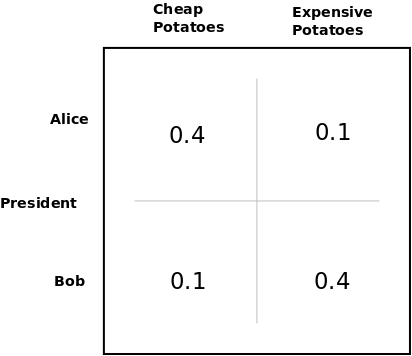
\includegraphics[width=\textwidth,height=6cm,keepaspectratio=true]{img/multidim-predictionmarket.png}
    \caption{Multidimensional prediction market.}
    \label{fig:potato}
\end{figure}

\paragraph{Multidimensional prediction markets}
Multidimentional prediction markets allow us to predict the correlation between possible future events.
So for example, one could predict that if Alice is elected leader, the price of potatoes will go down, and that if Bob wins, the price will go up. One could learn that if Google uses plan A for the next 3 months, that it will probably earn more money, and that if it uses plan B, it will probably earn less. Or, as in \cref{fig:potato}, we can see that if Alice would be elected president, there is a high likelihood of the price of potatoes being rather low.

\end{draft}

\begin{sketch}
\ifdraft
\subsubsection{Decentralized and trustless coin flip}
Each user commits to a single bit that is salted. If either user refuses to reveal, then they lose. The winner is determined by the XOR of the bits.

Assuming Casino and Gambler have a channel, the messages would go like this:
\begin{enumerate}
\item Gambler chooses a random bit, salts it, and sends the hash of it to Casino with a request to gamble.
\item Casino chooses a random bit, salts it, and uses the hash of it with the hash from Gamble to make the contract. Casino signs up for the contract and sends a copy back to Gambler.
\item Gambler signs the contract. Now the bet is live.
\item Gambler reveals the secret to Casino
\item Casino calculates the result, and sends its secret to Gambler with the new channel state. The new channel state doesn't include the bet, the aeon went to the winner.
\item Gambler calculates the result, and if they agree, then Gambler signs the new channel state.
\end{enumerate}


\subsubsection{Applications involving time}
Games like chess, poker, and go are popular for gambling. The timer measures time in seconds. To play the game we need to measure how long each player takes to make a turn, in seconds.
The blockchain consensus mechanism cannot measure time periods shorter than finality.
If someone somewhere makes a computer that signs over the current time every millisecond and publishes that data publicly, then we could use those signatures to make applications that enforce rules about time.
It would be best to put this computer onto a satellite orbiting the planet so that it is exceedingly difficult to extract the private key and sign on times ahead of schedule.
Channel applications can alternatively be programmed to follow the median of a handful of clocks. So if a minority of the clocks freeze, and/or a minority of clocks start publishing times ahead of schedule, our game still has the correct rules.
If the same clock system is used for many simultaneous games and markets, then a broken clock would make many applications break simultaneously. So the richest aeon holders are interested in maintaining a good clock, because a good clock increases the value of their aeon.
A good clock can also be profitable, if it charges users for signatures of the current time.
Channel contracts only get published in the event of disagreement, so the channel-users only need to buy signatures from the time-keeper if there is a disagreement. Thus, the use of the timer can be affordable and used to secure one's app. It will only charge one if one uses it.
\fi

\begin{draft}
\subsubsection{Market with batch trading at a single price}
There are two approaches available to attackers that want to rob aeon from a market. They can take advantage of the market being split in time, or they can take advantage of it being split in space.

\begin{itemize} 
   \item If the market is split in space, then the attacker does arbitrage. He simultaneously makes trades in both markets at once so that his risk cancels out and he earns a profit.
   \item If the market is split in time, then the attacker front-runs the market. He reads the transactions coming into the market and creates buy and sell orders immediately before and after.
\end{itemize}


\begin{figure}[htpb]
    \centering
    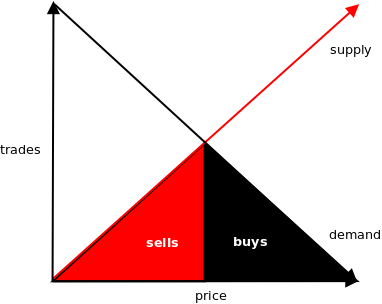
\includegraphics[width=\textwidth,height=6cm,keepaspectratio=true]{img/batch_channel.png}
    \caption{The black line is the demand curve, the red line is the supply curve. The sells in red are the same size as the buys in red. The vertical line is the price the market maker selected. Everyone willing to buy at a higher price traded at that price, everyone willing to sell at a lower price traded at that price.}
    \label{fig:batch_balanced}
\end{figure}

To combine markets in space, everyone should use the same market maker.
To combine markets in time, we need to have trading done in batches, at single price.
The market maker needs to commit to each person what price he decided, and if anyone can find contradictory commitments from the market maker, then all of his customers should be able to drain all of his channels.
If the market maker commits to a fair price, then he will match the same volume of buyers and sellers together, as \cref{fig:batch_balanced} shows. Otherwise, he will end up in a situation similar to \cref{fig:batch_unbalanced}, thus taking a large risk.

\begin{figure}[htpb]
    \centering
    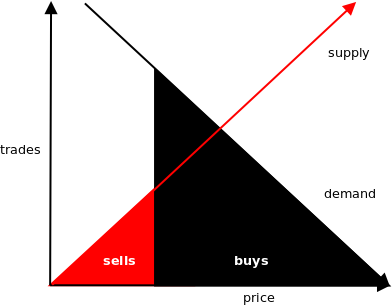
\includegraphics[width=\textwidth,height=6cm,keepaspectratio=true]{img/batch_channel_unbalanced.png}
    \caption{The black is much bigger than the red. The market maker is selling many more shares than it is buying, thus taking on a lot of risk.}
    \label{fig:batch_unbalanced}
\end{figure}


\end{draft}

\ifdraft      
\subsubsection{Spam filter}
Use channels to commit a safety deposit providing real non-spam, non-DDoS content \cite{ethereumpredictions}. If one does not like the content, then one does not unlock the spammer's safety deposit. 
   
      
\subsection{Non-blockchain applications}
For following applications no blockchain transactions are involved.
\subsubsection{Encrypted Messaging}
The public-private keys pair used for addresses and signing can also be used to create and receive encrypted (off-chain) messages. 
\subsubsection{Authentication}
Identities can also be used to authenticate against third-party web-services via signing a challenge.
\fi

\end{sketch}

\begin{draft}
\section{Implementation}
\label{sec:implementation}
Most key concepts already have proof-of-concept implementations in Erlang. This includes the blockchain itself, the contract language and VM, the oracle and governance mechanisms, as well as an old version of the consensus mechanism. We have used Erlang/OTP because it makes it easy to write code that can respond to many requests in parallel and does not crash. The servers with the highest up-time in the world are based on Erlang. It has been used for industrial applications for 30 years, proving itself to be a reliable and stable product.

\subsection{Virtual machine and contract language}
\label{sec:chalang}
The virtual machine is stack-based and similar to Forth and Bitcoin' scripting language, although in comparison to the latter, it is rather rich. The VM supports functions instead of gotos, making its semantics relatively simple to analyze. A list of the VM's opcodes can be found on our Github\footnote{\url{https://github.com/aeternity/chalang/blob/master/opcodes.md}}.

Additionally, there exists a higher-level Forth-like language called \textit{Chalang}, which compiles to bytecode for the VM. It supports macros and variable names, but keeps the stack-based execution model \cite{chalang}. Examples of Chalang code can also be found on our Github\footnote{\url{https://github.com/aeternity/chalang/tree/master/examples}}.

\subsection{Adoption via web-integration}
The web is the most popular application platform. We will provide easy-to-use web-development tools, such as JS-libraries and JSON-APIs for the core features of the Æternity blockchain. 
%Payment-channels will easily be established for API-requests, even the requests will be able to carry the Æternity channel transactions within them.

\subsection{Open source modules}
In order to be easily re-used for private blockchain consortium and other use-cases, the software will be written in MIT-licensed modules, such as a consensus module, that can be adapted to specific needs. 


\subsection{Usability and UX design}
Frictionless human interaction will be a big focus of our development efforts. More specifically, we will make sure that who controls the identity, keys and transactions is clearly established. Also, offering easy access via web-gateways will be a central focus of future development. Users participating in prediction markets via a Tinder-like (swipe left/right) mobile interface, and simple web-wallets that can be easily integrated in a website through an iframe will be the new norm.

\section{Discussion}
We have provided an explanation of how to architect a fundamentally more efficient value transfer system. The described system is in fact a global oracle machine that can be used to provide decision making services at global scale. In particular, all the applications proposed in \cref{sec:applications} can be built easily and efficiently on top of Æternity.

However, our approach has both fundamental limitations and avenues for improvement. These are discussed here. 

\subsection{Limitations and tradeoffs}
While we do believe that the tradeoffs made in our architecture are reasonable given the resulting performance increase in other areas, Æternity is not a catch-all solution for decentralized applications. It should rather be viewed as a synergistic complement to existing technologies. There are several caveats that one need to be aware of.

\subsubsection{On-chain state}
Despite having many advantages, Æternity's lack of programmable state makes it unfit for applications that require a custom state to be under consensus. For example, this includes DAOs as they are usually conceived, custom name systems and subcurrencies which are not tied to the value of an underlying asset.

\subsubsection{Free option problem}
If Alice and Bob have a channel and Alice signs a contract, she essentially gives Bob a free option when she sends it to him: Bob can choose to sign and return (i.e. activate) the contract at any time in the future. Often this is not what is intended. To avoid this problem, channel contracts aren't immediately activated with the full amount. They are divided up in time or space. Both participants would sign up for the contract in small intervals so that neither user ever offers a large free option to the other.

For example, if the parties want to bet 100 aeon, then they might sign up to it in 1000 steps that each increase the bet by 0.1 aeon. This would require about 1000 messages to pass, 500 in each direction, which is cheap enough since the contract is never submitted to the blockchain. As another example, if one wanted to make a financial asset that would last for 100 days, one might sign up in 2400 steps of one hour each. This would require about 2400 messages to pass, 1200 in each direction.

\subsubsection{Liquidity loss and state channel topologies}
When composing channels using hashlocks as demonstrated in \cref{sec:contracts}, any middlemen have to lock up at least twice as many aeon as will be transmitted through them. For example, if Alice and Carol want to transact through Bob, Bob will act as Carol when interacting with Alice, and vice-versa.

Since this is expensive for Bob, he would most likely earn a fee as compensation. If Alice and Carol expect to conduct many trades between each other, they can avoid this by creating a new channel and trustlessly moving the active contracts to the new channel using a hashlock.

Still, since keeping an extra channel open impacts one's liquidity negatively, going through middlemen is expected to be desirable in many cases, especially in cases where the parties don't expect to trade a lot in the future. Thus, a channel topology where certain rich users make money from trustlessly transmitting transactions between other users is expected to emerge.

It should be noted that this does not constitute a single point of failure, since we do not trust these transaction transmitters with anything. If a transmitter goes offline before the secret to a hashlock has been revealed, the transaction doesn't go through. If it goes offline afterwards, the only possible ``negative'' effect is that the transmitter is not able to claim its aeon.

\subsection{Future work}
There are several possible ways to improve on the current architecture.

\ifdraft
\subsubsection{Improving the oracle}
\sk{Zack talked about how we could measure beliefs instead of desires. Worth mentioning?}
\fi

\subsubsection{Functional contract language}
\begin{draft}
A reasonable future direction would be to experiment with high-level languages that adhere more closely to the functional paradigm. Keeping track of an implicit stack is generally error-prone and arguably not suitable for a high-level, developer-facing language. This should be rather easy given that programs are already pure functions (modulo some environment variables), and would greatly simplify both development and formal verification of contracts. If this is done, it could also make sense to revise the VM to be tightly coupled with the new language, to make the compilation less error-prone and less dependent on trust in the developers. Ideally, the translation from surface language to VM code would simply be a direct transcription of peer-reviewed research, though pragmatic concessions will likely have to be made.
\end{draft}


\subsubsection{Multi-party channels}
Currently, all channels on Æternity are limited to two parties. While multi-party channels can \emph{de facto} be achieved through hashlocking, this can be expensive. Hence, we plan to investigate the possibility of adding support for $n$-party channels, with a $m$-of-$n$ settlement mechanism.

\ifdraft
\subsubsection{Futarchy}
Futarchy is a governance system devised by economist Robin Hanson, in which elected officials define metrics of national welfare that should be maximized, and prediction markets are used to determine which policies will have the most positive effect with respect to these measures \cite{futarchy}. While Æternity's governance system potentially uses both voting and prediction markets, it is not a futarchy. This is because the votes are not used to determine a metric, but to govern the system directly. In fact, there is not even any globally accepted metric that should be optimized; every user chooses for themselves what they want to optimize, and may ask prediction market(s) how to they should vote to do this.
\fi

\end{draft}

\section*{Glossary}
\begin{LaTeXdescription}
\item[Blockchain] A distributed, tamper-proof database with metered access. The database is defined by a growing list of hash-linked blocks and can have any rules for appending them.
\item[Aeon] An aeon represents a unit of account and an access right to the Æternity blockchain. It is transferable.
\item[Transaction] A message from a user to the blockchain. This is how users can use their currency to access the blockchain.
% \item[Vote] This is the transaction type that value-holders can use to participate in the consensus mechanism.
\item[State Channel] A relationship between two users recorded on the blockchain. It enables users to send aeon back and forth, and to create trustless smart contracts between them that are enforced and settled by the blockchain.
\item[Hash] A hash takes as input a binary of any size. It gives a fixed sized output. The same input always hashes to the same output. Given an output, one cannot calculate the input.
\item[Hashlocking] This is how we connect pairs of channels to make smart contracts that involve more than 2 people. A secret is referenced by it's hash. When the secret is revealed, it can update multiple channels at the same time.
\item[Governance] A well-defined process of making decisions for the future protocol(s) of the blockchain.
\item[Oracle] A mechanism that tells the blockchain facts about the world we live in. Using oracles users can predict the outcome of events, external to the blockchain system.
\item[Value-Holder] A user who owns aeon, or a financial derivative in the system.
\item[Validator] A validator is a user who participates in the consensus mechanism. In the case of Æternity, every value-holder can participate.
\end{LaTeXdescription}

\iffalse
\section{TODO}
\subsection{Terms to decide and find+replace}

\begin{itemize} 
   % \item "vote tree" vs "vote-tree"
   \item information-, prediction-, vs event-markets
   \item "smart contract" vs "smart-contract"
   \item users/nodes as "it" vs "he" vs "she" vs "they"
   \item "time frame" vs "timeframe" vs time-frame (Zack thinks one word is better than two)
   \item "Æternity" vs "Aeternity"
   \item "aeon" vs "æon"
\end{itemize}

\subsection{Other}
\begin{itemize}
\item (incomplete) list of variables for governance (votes)? > 
\item add scalability calculations
\item discuss term 'bribe'
\item discuss vote key <-- priv key (so that priv keys can stay offline) (this can be done with HD-keys, right?)
\item move oracle disputes into governance? discuss difference between governance and consensus. 
\item Change all "" to ``''
\end{itemize}

\fi


%\section*{APPENDIX}


\section*{ACKNOWLEDGMENTS}
Thanks to Vlad, Matt, Paul, Dirk, Martin, Alistair, Devon and Ben for proof-reading. Thanks to these and lots of other people for insightful discussions.
%Vlad: I will be happy if you include me here as a reviewer.

%\bibliographystyle{plain}
%\bibliography{references.bib}

%\addcontentsline{toc}{chapter}{References}
%\input{include/backmatter/References}
%\bstctlcite{IEEEexample:BSTcontrol}
\printbibliography



\end{document}
